\documentclass[12pt]{article}
\usepackage{graphicx}
\graphicspath{ {./graphs/} }
\usepackage{color}
\usepackage{url}
\usepackage[a4paper, total={6in, 8in}]{geometry}

\begin{document}

\title{COL 334/672 – Semester II 2023-24: Assignment 3 \\ Milestone 2 Report}
\author{Parth Thakur, 2021CS50615\\ Amish Kansal, 2021CS50622}
\date{\today}
\maketitle

\section{Introduction}
This report presents our findings and results for Milestone 2 of Assignment 3. We have implemented a UDP client for reliably transferring data from a server, which mimics TCP's congestion control behavior.

\section{Client Implementation}

We have implemented two types of clients:
\begin{itemize}
    \item AIMD (Additive Increase, Multiplicative Decrease) client
    \item Fixed burst size client
\end{itemize}

\subsection{AIMD Client}
Our AIMD client sends requests in bursts. The size of these bursts is varied using an AIMD strategy. If all requests in a burst are successfully received, the burst size is incremented by one for the next burst. If some requests are not received, the burst size is halved.

\subsection{Fixed Burst Size Client}
We implemented clients with fixed burst sizes of 4 and 10. These clients send requests in bursts of their respective sizes without any adjustments based on network feedback.

\clearpage
\section{Experimental Results}

\subsection{AIMD Client}

Figures \ref{fig:aimd1}, \ref{fig:aimd2}, and \ref{fig:aimd3} depict the performance and behavior of our AIMD client.


\begin{figure}[h]
    \centering
    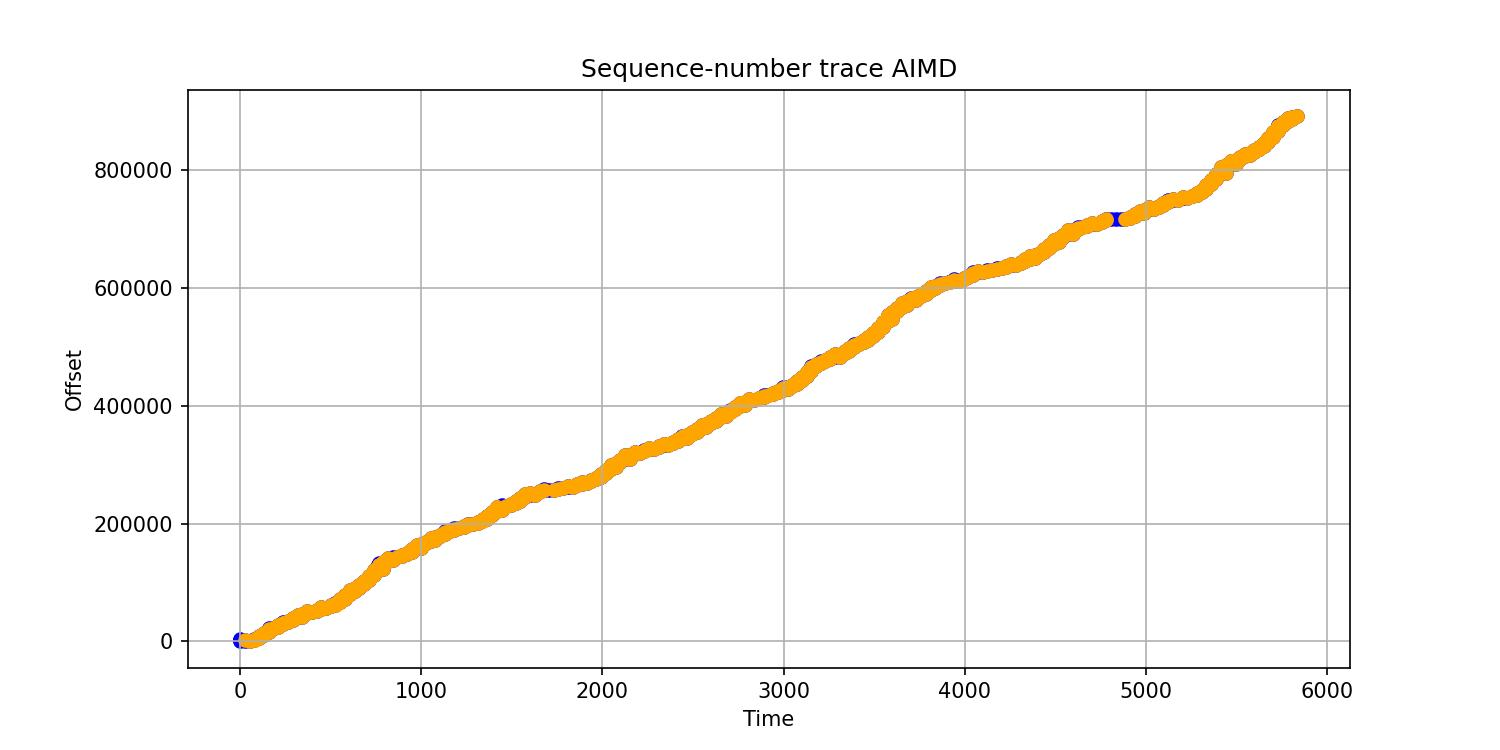
\includegraphics[width=0.7\linewidth]{AIMD_1.jpeg}
    \caption{Performance graph for AIMD client (part 1)}
    \label{fig:aimd1}
\end{figure}

\begin{figure}[h]
    \centering
    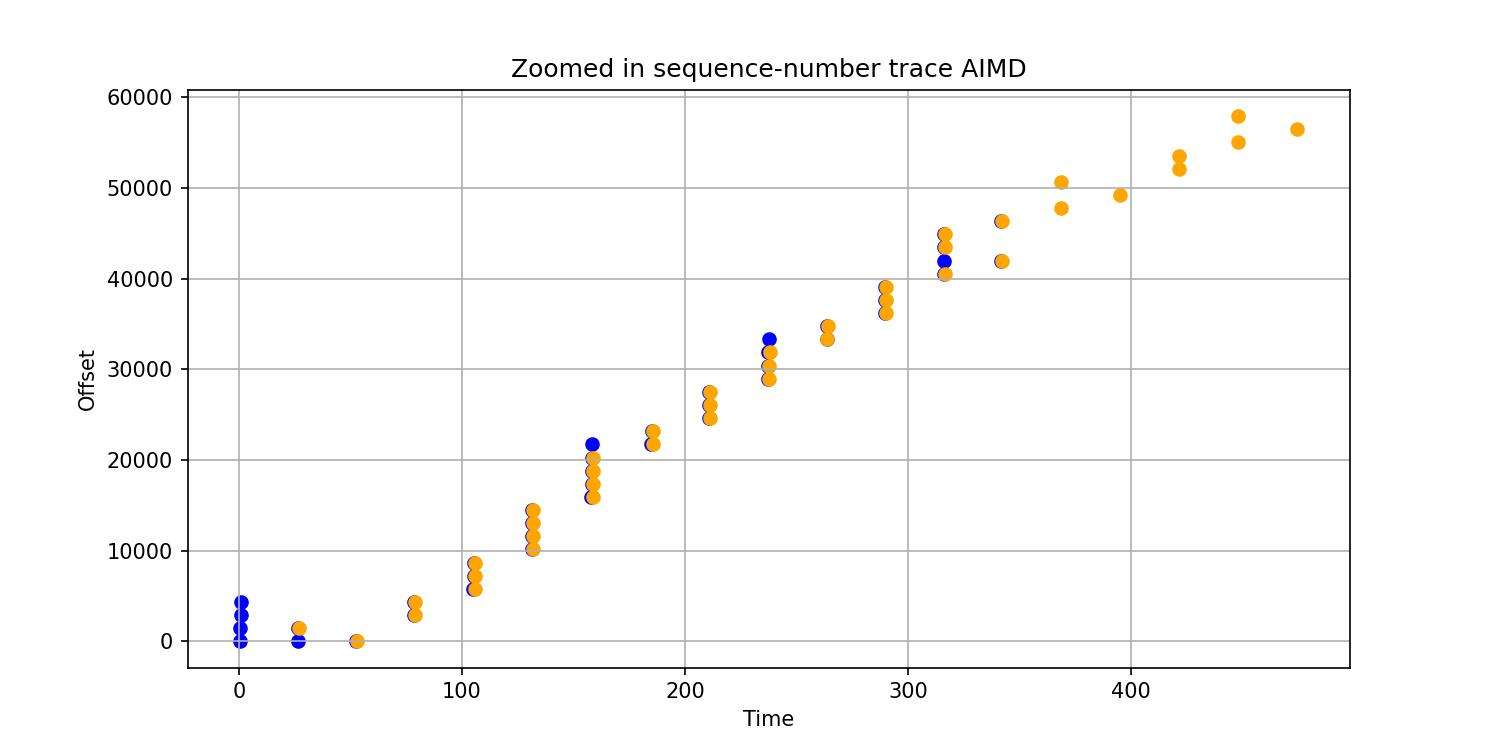
\includegraphics[width=0.7\linewidth]{AIMD_2.jpeg}
    \caption{Zoomed performance graph for AIMD client (part 2)}
    \label{fig:aimd2}
\end{figure}

\begin{figure}[h]
    \centering
    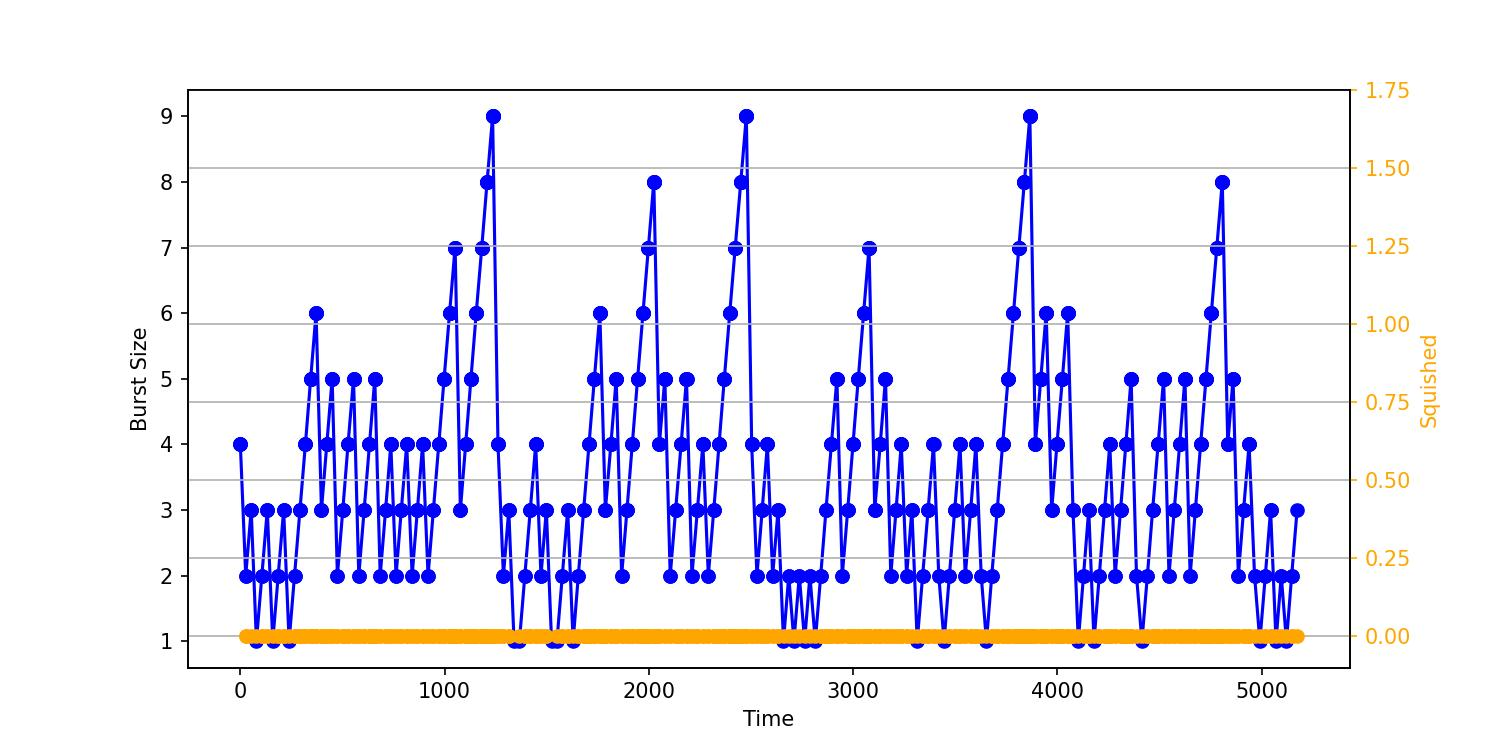
\includegraphics[width=0.7\linewidth]{AIMD_3.jpeg}
    \caption{Burst size vs time graph for AIMD client (part 3)}
    \label{fig:aimd3}
\end{figure}

\clearpage
\subsection{Fixed Burst Size Client (Size 4)}

Figures \ref{fig:fixed4_1}, \ref{fig:fixed4_2}, and \ref{fig:fixed4_3} depict the performance and behavior of our fixed burst size client with a burst size of 4.

\begin{figure}[h]
    \centering
    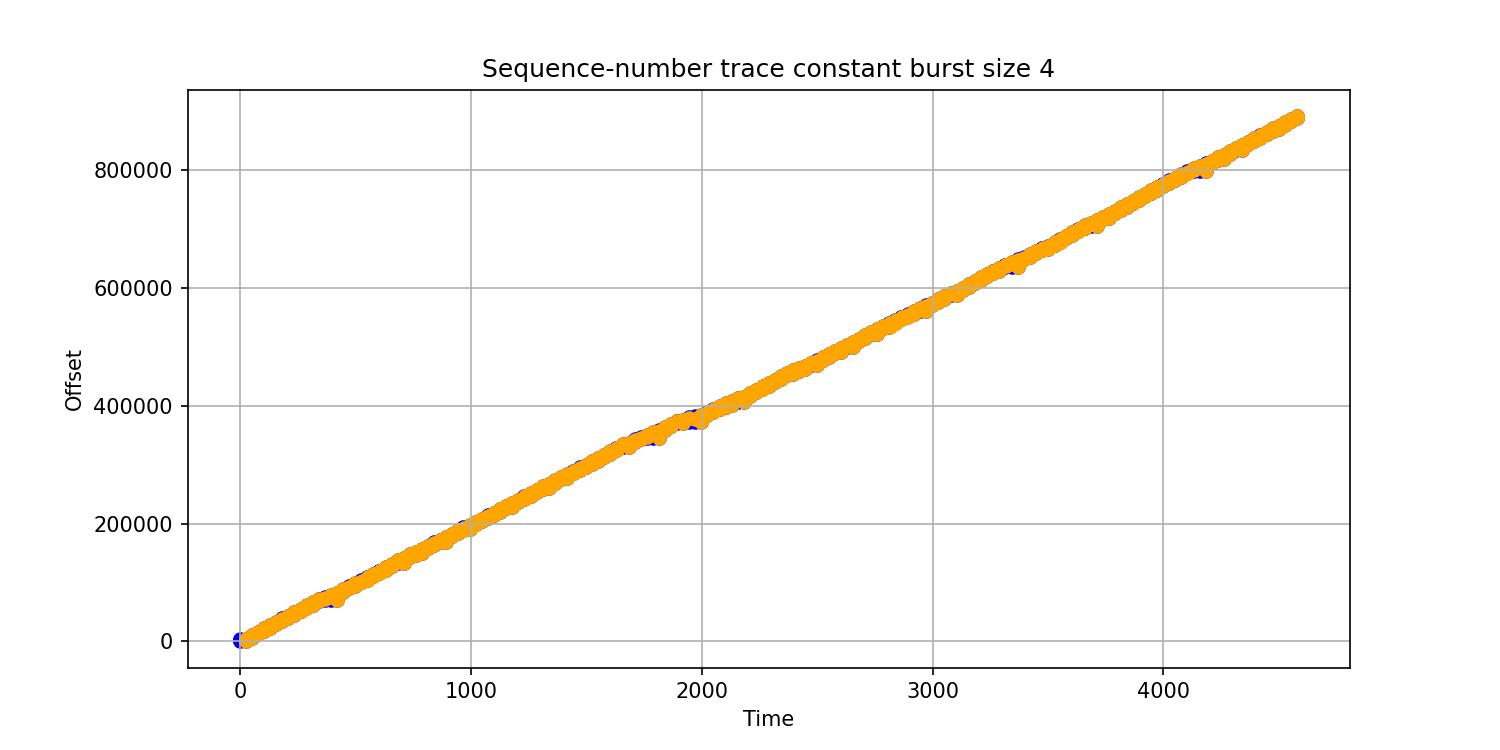
\includegraphics[width=0.7\linewidth]{constant burst size 4_1.jpeg}
    \caption{Performance graph for fixed burst size client (size 4, part 1)}
    \label{fig:fixed4_1}
\end{figure}

\begin{figure}[h]
    \centering
    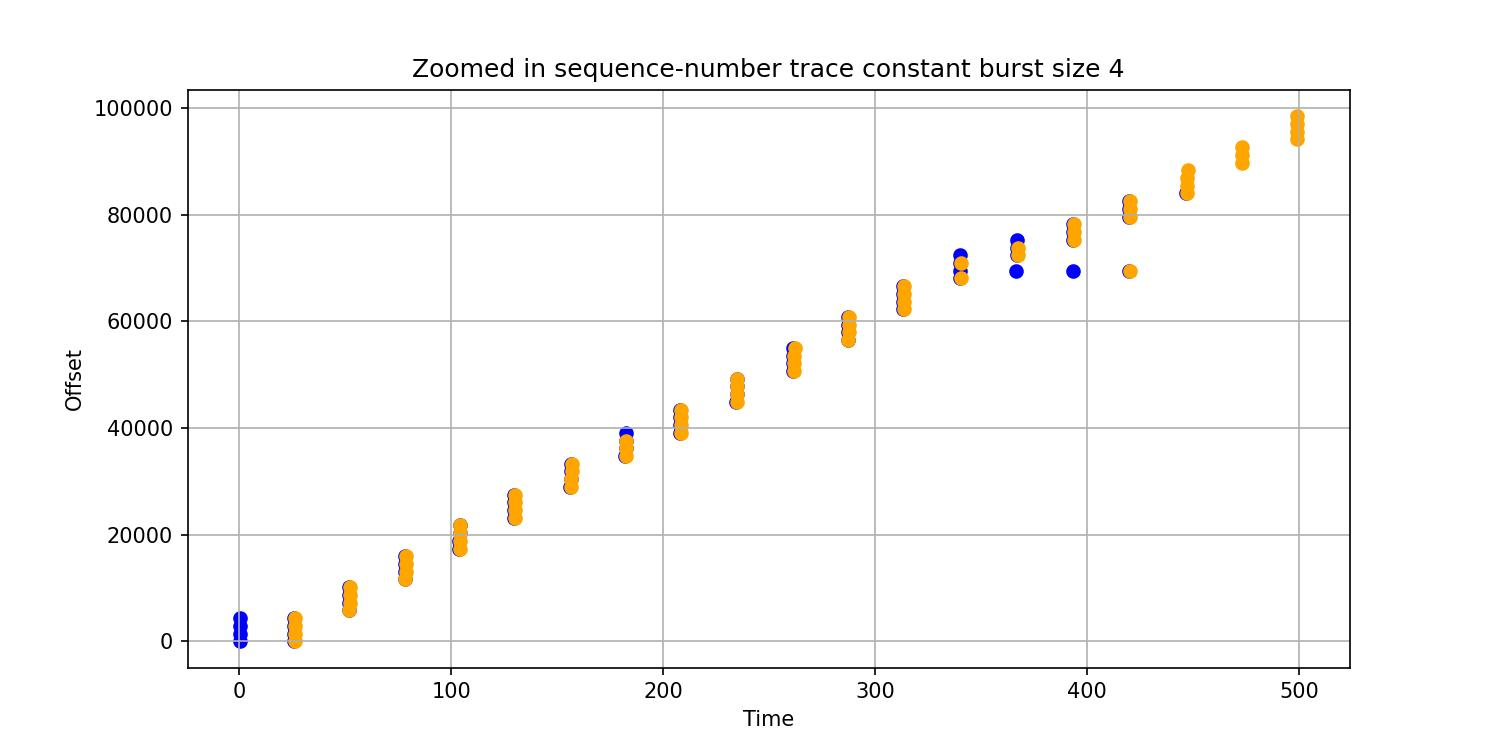
\includegraphics[width=0.7\linewidth]{constant burst size 4_2.jpeg}
    \caption{Performance graph for fixed burst size client (size 4, part 2)}
    \label{fig:fixed4_2}
\end{figure}

\begin{figure}[h]
    \centering
    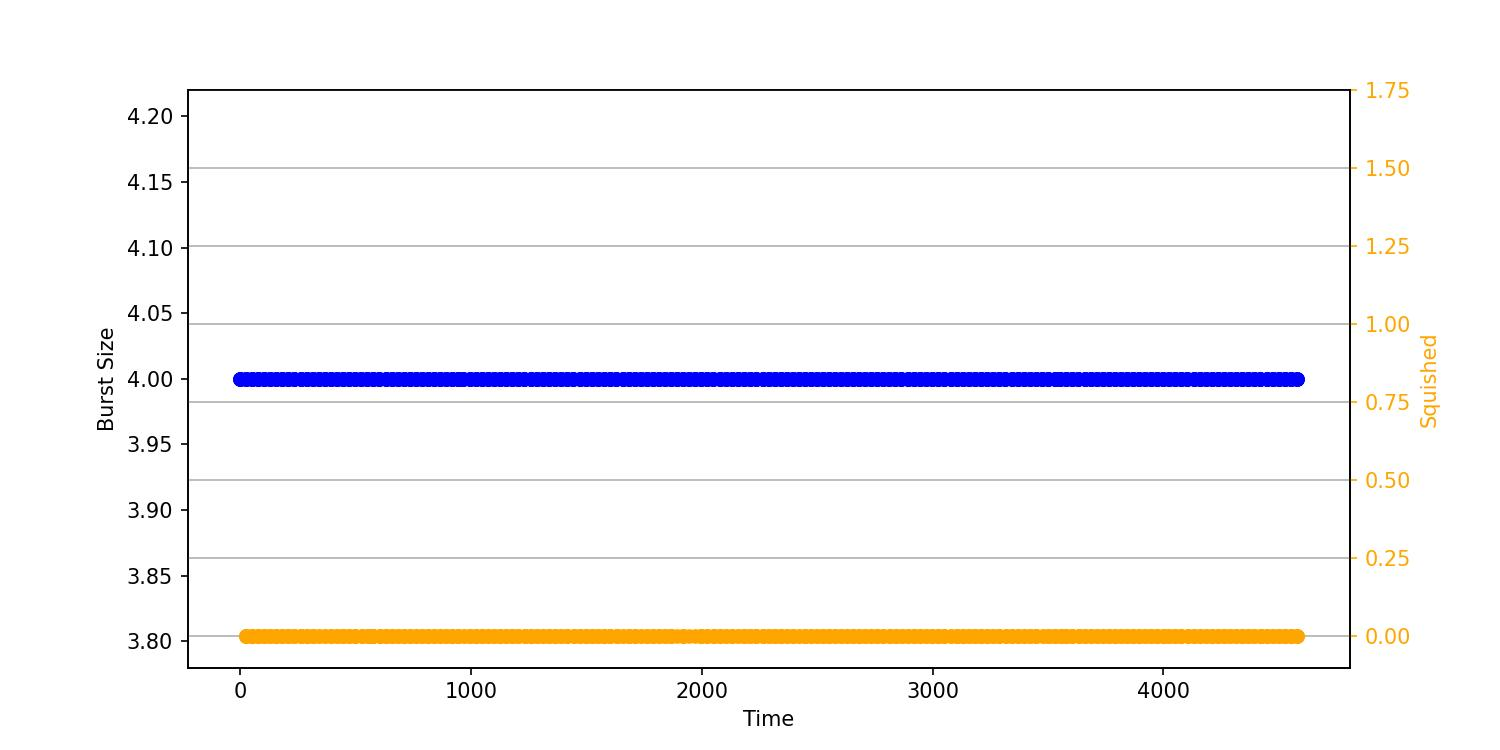
\includegraphics[width=0.7\linewidth]{constant burst size 4_3.jpeg}
    \caption{Performance graph for fixed burst size client (size 4, part 3)}
    \label{fig:fixed4_3}
\end{figure}

\clearpage
\subsection{Fixed Burst Size Client (Size 10)}

Figures \ref{fig:fixed10_1}, \ref{fig:fixed10_2}, and \ref{fig:fixed10_3} depict the performance and behavior of our fixed burst size client with a burst size of 10.

\begin{figure}[h]
    \centering
    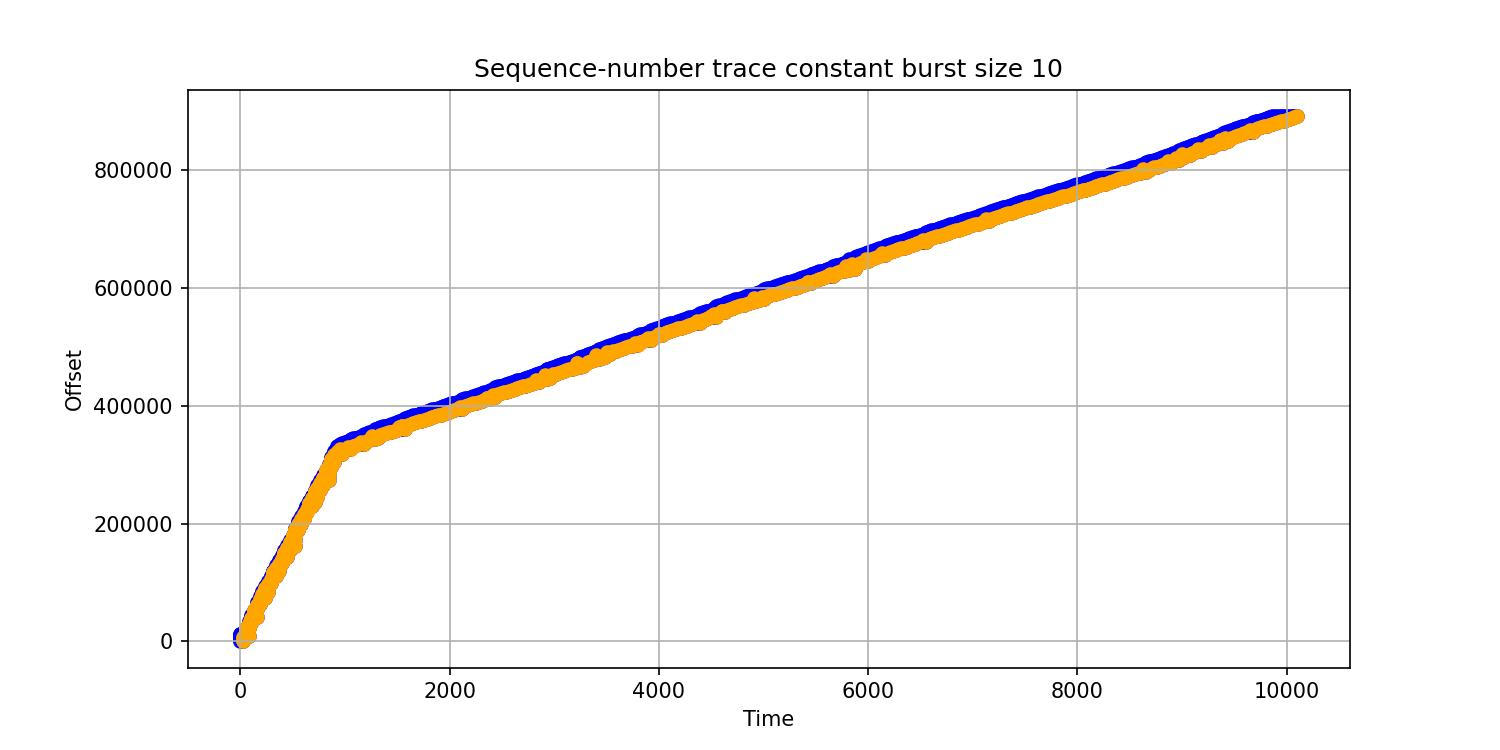
\includegraphics[width=0.7\linewidth]{constant burst size 10_1.jpeg}
    \caption{Performance graph for fixed burst size client (size 10, part 1)}
    \label{fig:fixed10_1}
\end{figure}

\begin{figure}[h]
    \centering
    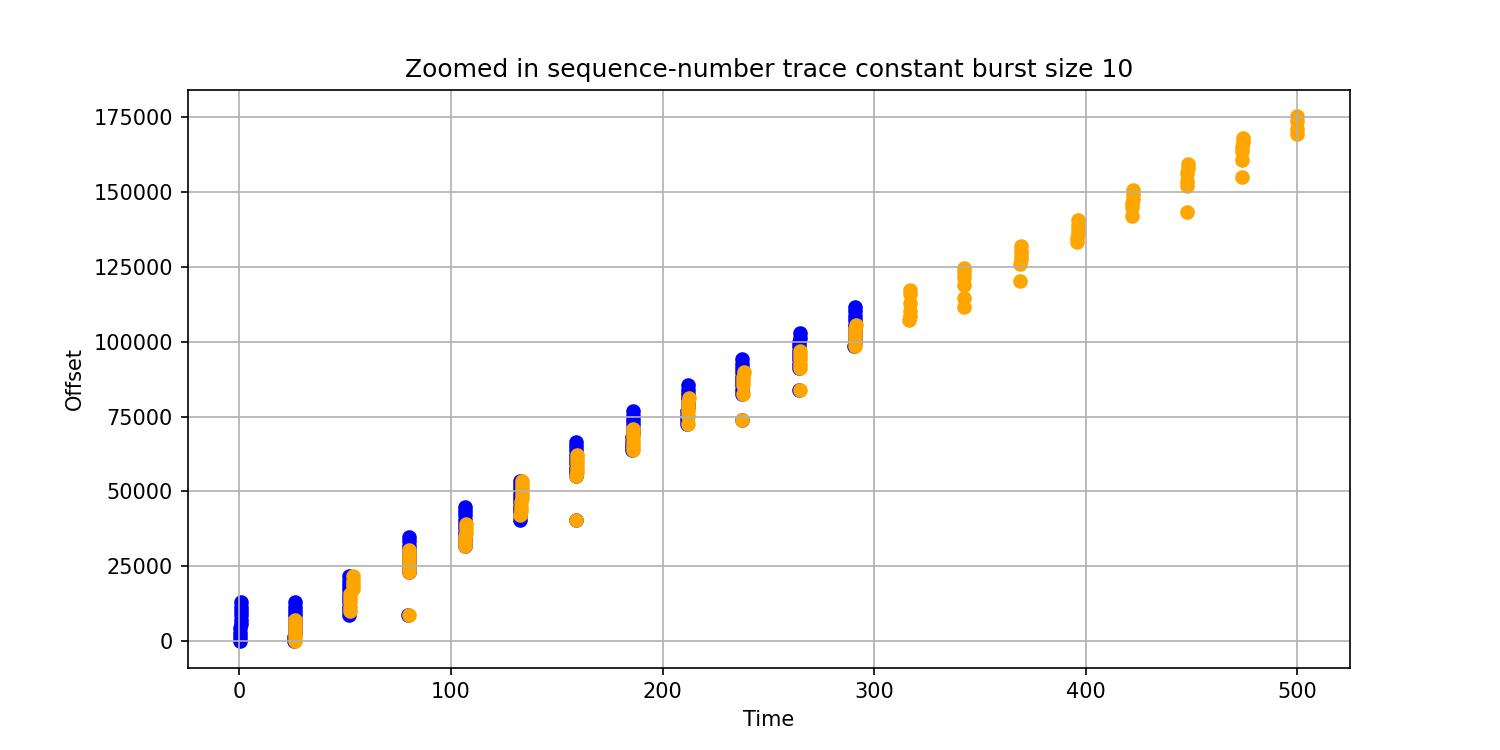
\includegraphics[width=0.7\linewidth]{constant burst size 10_2.jpeg}
    \caption{zoomed in performance graph for fixed burst size client (size 10, part 2)}
    \label{fig:fixed10_2}
\end{figure}

\begin{figure}[h]
    \centering
    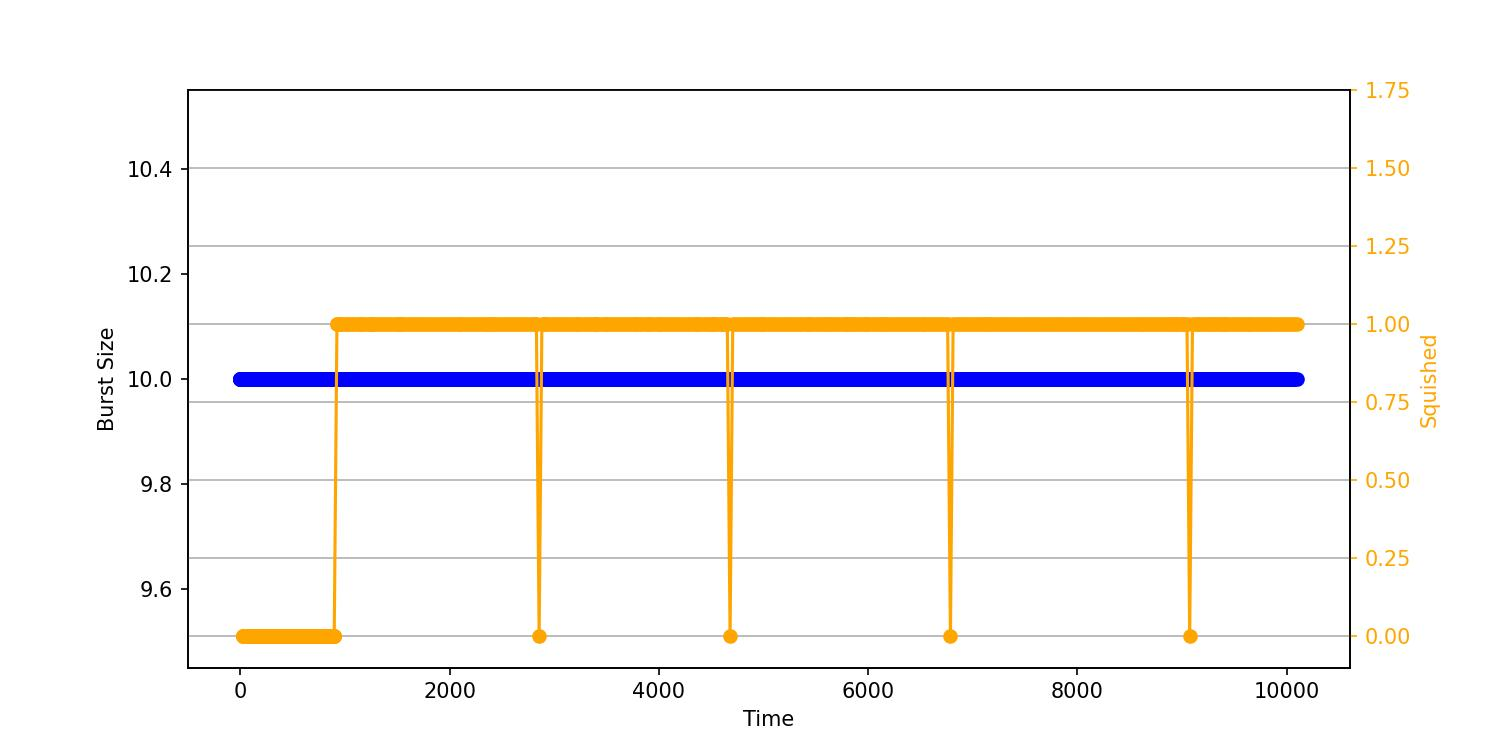
\includegraphics[width=0.7\linewidth]{constant burst size 10_3.jpeg}
    \caption{Burst size vs time graph for fixed burst size client (size 10, part 3)}
    \label{fig:fixed10_3}
\end{figure}

\clearpage
\section{Conclusion}
Through our experiments, we observed that the AIMD client is adaptive to network conditions, while the fixed burst size client's performance remains consistent. The adaptive nature of the AIMD client ensures better utilization of available bandwidth and reduces the risk of network congestion.

\end{document}
